\documentclass{article}
\usepackage{amssymb}
\usepackage{amsmath}
\usepackage{graphicx} % Required for inserting images
\usepackage[a4paper, total={7in, 10in}]{geometry}

\newcommand\cha{3}

\title{Mini Ep 5 - Otimizando o uso de cache - parte 1}
\author{Paulo Henrique Albuquerque, NUSP:12542251}
\date{2023-04-27}

\begin{document}

\maketitle

\section{Diferença dos tempos dos algoritmos}

O algorimo otimizado apresentou melhora do tempo de execução. Em particular, o programa teste dá resultado positivo:

\begin{figure}[htpb]
  \centering
  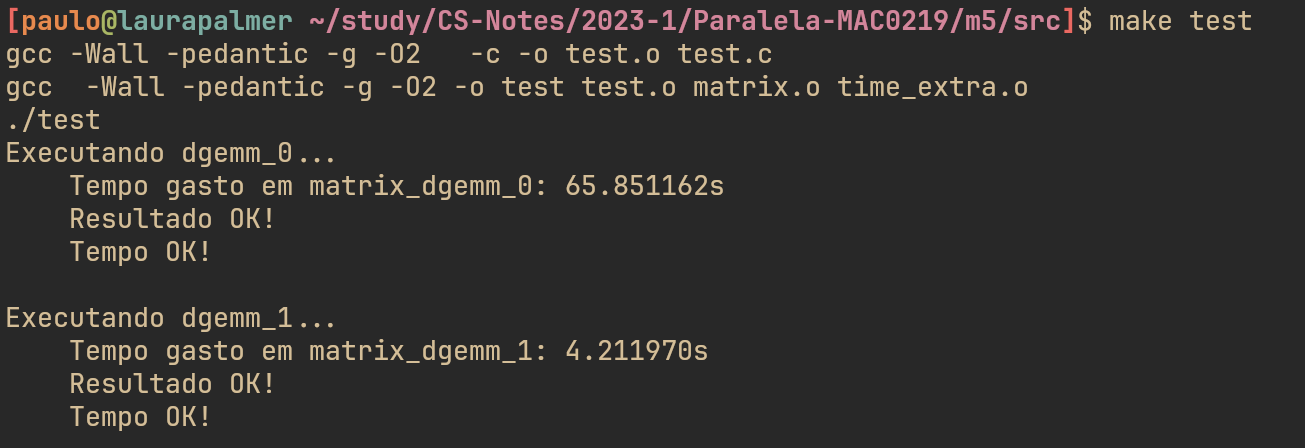
\includegraphics[width=0.8\textwidth]{teste.png}
  \caption{teste.png}
  \label{fig:teste-png}
\end{figure}

Para compararmos os tempos de execução, executamos os dois algoritmos para vários tamanhos $N$ das matrizes. Para cada instância, foi rodado cada algoritmo 5 vezes e tirado a média simples dos tempos de execução. O tempo foi medido usando o programa main fornecido e o script para realizar a média foi o seguinte:

\begin{figure}[htpb]
  \centering
  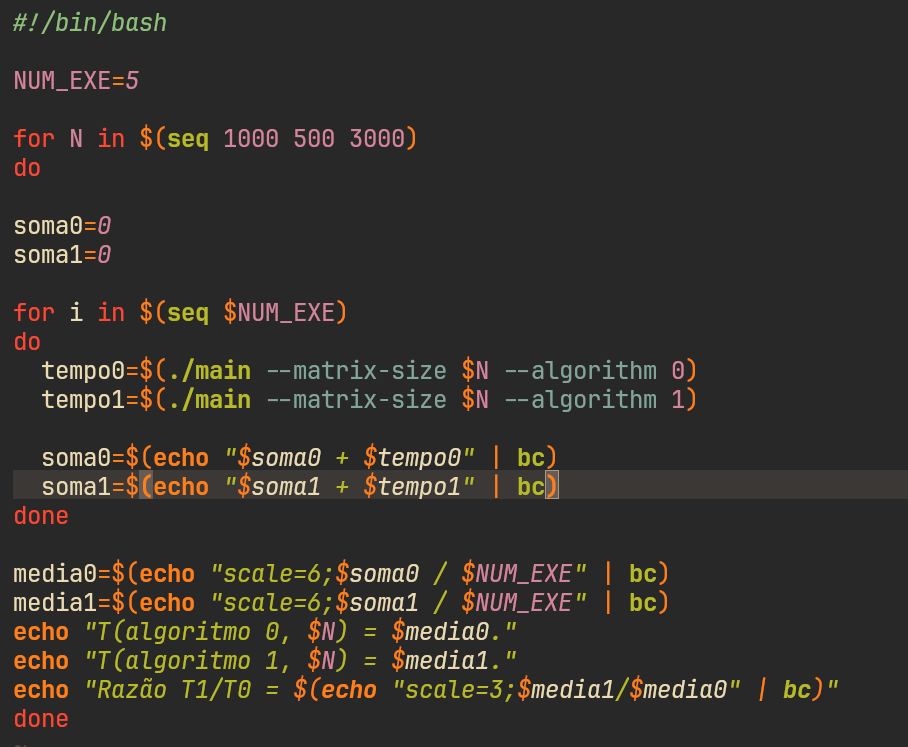
\includegraphics[width=0.8\textwidth]{script.png}
  \caption{script.png}
  \label{fig:script-png}
\end{figure}

Os resultados são mostrados na figura abaixo. 

\begin{figure}[htpb]
  \centering
  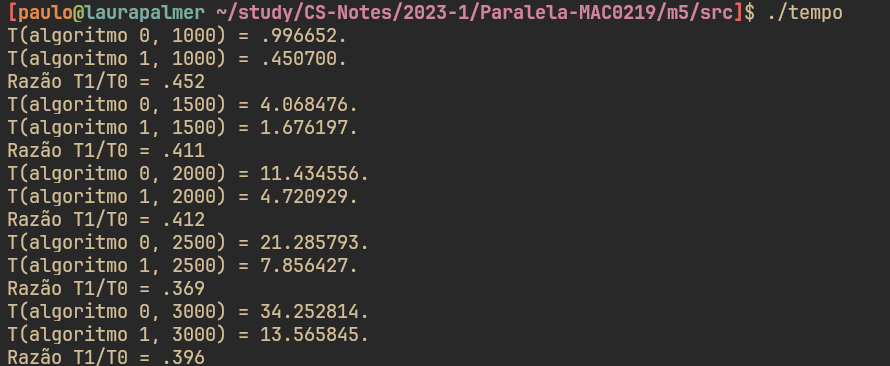
\includegraphics[width=0.8\textwidth]{resultados.png}
  \caption{resultados.png}
  \label{fig:resultados-png}
\end{figure}

A tabela abaixo resume os resultados.

Como podemos ver pelos resultados acima, é nitída a melhora no tempo de execução: o algortimo otimizado foi mais rápido que o algortimo simples cerca de 4 vezes nos testes.

\subsection{Explicação do algoritmo otimizado}

O algoritmo otimizado consiste em alterar a ordem dos laços do algoritmo simples a fim de se aproveitar da memória cache para tornar os acessos às entradas das matrizes mais rápidos. No algorimo simples, a ordem os laços é,

\begin{figure}[htpb]
  \centering
  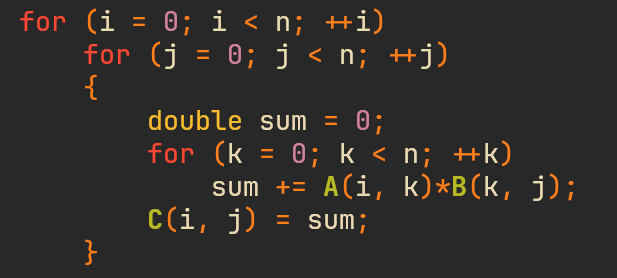
\includegraphics[width=0.8\textwidth]{simples.png}
  \caption{simples.png}
  \label{fig:simples-png}
\end{figure}

enquanto no algoritmo otimizado é,


\begin{figure}[htpb]
  \centering
  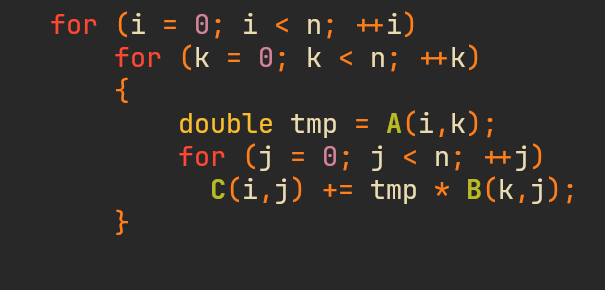
\includegraphics[width=0.8\textwidth]{otimizado.png}
  \caption{otimizado.png}
  \label{fig:otimizado-png}
\end{figure}

A correção do algoritmo é simples e não será feita com detalhes aqui. Basicamente, o algoritmo percorre as linhas da matriz $A$ e da matriz $B$. Isso é feito porque quando acessamos um elemento de uma matriz na mémoria, outros elementos da mesma linha são trazidos para o cache. Então, como no algoritmo de multiplicação de matrizes simples percorremos as colunas de $B$, trazer outros elementos da mesma linha de $B$ é inútil e obtemos vários caches miss. No algoritmo otimizado, isso é mitigado pois percorremos linhas de $B$. Além disso, note que o elemento de $A$ que será utilizado dentro do laço mais interno é armazenado em um variável temporária. Dessa forma, não precisamos acessar a memória toda vez que fizermos a atualização $C(i,j) +=\ldots$.

\section{Diferentes Maquinas}



\end{document}
